%-------------------------------------------------------------------------%
%--------------------Classroom Lecture Model Series-----------------------%
%-------------------------------------------------------------------------%
\documentclass[preprint, 8pt]{elsarticle}
\usepackage{xcolor}
\usepackage{chemfig}
\usepackage{tikz}
\usepackage{graphicx}
\usepackage{amsmath, amssymb}
\setlength{\parindent}{0pt}
\usepackage{pgfplots}
\pgfplotsset{compat=1.3,}
\pgfplotscreateplotcyclelist{line styles}{ 
	black,solid\\
	blue,dashed\\
	red,dotted\\
	orange,dashdotted\\
}
\newcommand*\GnuplotDefs{
	set samples 50;
	cdfn(x,mu,sd) = 0.5 * ( 1 + erf( (x-mu)/sd/sqrt(2)) );
	pdfn(x,mu,sd) = 1/(sd*sqrt(2*pi)) * exp( -(x-mu)^2 / (2*sd^2) );
	tpdfn(x,mu,sd,a,b) = pdfn(x,mu,sd) / ( cdfn(b,mu,sd) - cdfn(a,mu,sd) );
}
\usepackage[a4paper,bindingoffset=0.2in,
left=0.5in,right=0.5in,top=1in,bottom=1in,
footskip=.25in]{geometry}
%\usepackage{geometry}
\usepackage{mathtools}
\usepackage{tkz-berge}
\usetikzlibrary{calc} 
\usetikzlibrary{automata}
\usetikzlibrary{arrows}
\usetikzlibrary{positioning,shapes,shadows,arrows}
\usetikzlibrary{shapes.geometric}
\usetikzlibrary{calendar,shadings}
\renewcommand*{\familydefault}{\sfdefault}
\colorlet{winter}{blue}
\colorlet{spring}{green!60!black}
\colorlet{summer}{orange}
\colorlet{fall}{red}
\newcount\mycount
\newcommand\shapeLarge{50mm}
\newcommand\shapeMedium{25mm}
\newcommand\shapeSmall{5mm}
\newcommand*{\xMin}{0}
\newcommand*{\xMax}{6}
\newcommand*{\yMin}{0}
\newcommand*{\yMax}{6}
\newcommand*{\zMax}{6}
\newcommand*{\zMin}{0}
\definecolor{colorwaveA}{RGB}{98,145,224}
\definecolor{colorwaveB}{RGB}{250,250,50}
\definecolor{colorwaveC}{RGB}{25,125,25}
\definecolor{colorwaveD}{RGB}{100,100,100}
\definecolor{colorwaveE}{RGB}{80,100,1}
\definecolor{colorwaveF}{RGB}{60,1,1}
\definecolor{colorwaveG}{RGB}{25,1,100}
\definecolor{colorwaveH}{RGB}{1,90,1}
\definecolor{colorwaveI}{RGB}{1,100,1}
\definecolor{colorwaveJ}{RGB}{1,1,1}
\tikzset{
	shapeTriangle/.style={draw,shape=regular polygon,fill=colorwaveA,circular drop shadow,regular polygon sides=3,minimum size=\shapeSmall,inner sep=0pt,outer sep=0pt},
	shapeTriangle3/.style={shapeTriangle,fill=colorwaveD,circular drop shadow,shape border rotate=45},
	shapeTriangle4/.style={shapeTriangle,fill=colorwaveA,circular drop shadow,shape border rotate=90},
	shapeTriangle5/.style={shapeTriangle,fill=colorwaveB,shape border rotate=135},
	shapeTriangle6/.style={shapeTriangle,fill=colorwaveC,shape border rotate=180},
	shapeTriangle7/.style={shapeTriangle,fill=colorwaveE,shape border rotate=225},
	shapeTriangle8/.style={shapeTriangle,fill=colorwaveF,shape border rotate=270},
	shapeTriangle9/.style={shapeTriangle,fill=colorwaveG,shape border rotate=315},
}

\tikzset{
	shapeSquare/.style={draw,shape=regular polygon,fill=colorwaveC,circular drop shadow,regular polygon sides=4,minimum size=\shapeSmall,inner sep=0pt,outer sep=0pt},
	shapeSquare2/.style={shapeSquare,shape border rotate=45},
}

\tikzset{
	shapeHexagon/.style={draw,shape=regular polygon,fill=colorwaveA,circular drop shadow,regular polygon sides=6,minimum size=\shapeSmall,inner sep=0pt,outer sep=0pt},
	shapeHexagon2/.style={shapeHexagon,shape border rotate=90},
}

\tikzset{
	shapeOctagon/.style={draw,shape=regular polygon,fill=colorwaveB,circular drop shadow,regular polygon sides=8,minimum size=\shapeSmall,inner sep=0pt,outer sep=0pt},
	shapeOctagon2/.style={shapeHexagon,shape border rotate=45},
}
\tikzset{
	shapeEllipse/.style={draw,shape=ellipse,minimum size=\shapeSmall,inner sep=0pt,outer sep=0pt},
	shapeEllipse2/.style={shapeEllipse,shape border rotate=90},
}

\tikzset{
	closedFigure/.style={draw=\draw[->,rounded corners=0.2cm,shorten >=2pt]
		(1.5,0.5)-- ++(0,-1)-- ++(1,0)-- ++(0,2)-- ++(-1,0)-- ++(0,2)-- ++(1,0)--
		++(0,1)-- ++(-1,0)-- ++(0,-1)-- ++(-2,0)-- ++(0,3)-- ++(2,0)-- ++(0,-1)--
		++(1,0)-- ++(0,1)-- ++(1,0)-- ++(0,-1)-- ++(1,0)-- ++(0,-3)-- ++(-2,0)--
		++(1,0)-- ++(0,-3)-- ++(1,0)-- ++(0,-1)-- ++(-6,0)-- ++(0,3)-- ++(2,0)--
		++(0,-1)-- ++(1,0)}
}
\tikzstyle{start}=[circle, draw=none,,minimum size=\shapeMedium, fill=blue, circular drop shadow,text centered, anchor=north, text=white]
\tikzstyle{finish}=[circle, draw=none,,minimum size=\shapeMedium, fill=blue,circular drop shadow,text centered, anchor=north, text=white]
\tikzstyle{finish}=[rectangle, draw=none, ,minimum size=\shapeMedium,fill=blue,circular drop shadow,text centered, anchor=north, text=white]
\usepackage[noadjust]{cite}
\usepackage{algpseudocode}
\usepackage{listings}
\usepackage{algorithm}
\usepackage{color}
\usepackage{parskip}
\usepackage{amsfonts}
\usepackage{amsthm}
\usepackage{tikz}
\usepackage{tkz-berge}
\usepackage{caption}
\usepackage{hyperref}
\usepackage{amsrefs}
\usepackage{mathtools, amssymb}
\usepackage{graphicx}
\usepackage{subcaption}
\usepackage{tabularx,ragged2e}
\usepackage[framemethod=tikz]{mdframed}
\newcommand{\N}{\mathbb N}
\newcommand{\Q}{\mathbb Q}
\theoremstyle{definition}
\newtheorem{definition}{Definition}[section] 
\newtheorem{theorem}{Theorem}[section]
\newtheorem{example}{Example}[section]
\renewcommand{\qedsymbol}{$\blacksquare$}
\newtheorem{corollary}{Corollary}[theorem]
\newtheorem{lemma}[theorem]{Lemma}
\renewcommand{\rmdefault}{ptm} 
\graphicspath{{Figures/1/}}
\twocolumn
\begin{document}
\begin{frontmatter}
		\title{Course 1 Lecture 1 Journal Article 1:  DRAFT Sample: DNA Shape Categories for Statistical Learning Models of Gene Overexpression, Amplification, Mutation and Regulation in GastroIntestinal Cancers}
		\author{TMLS \corref{cor1}\fnref{fn1}}
		\cortext[cor1]{Corresponding author}
		\address{}
		\ead{}	
\end{frontmatter}	
Abstract:
	
\textbf{Introduction: . }
Objective 1: 
Objective 2: 
Objective 3: 
\textbf{Conclusion:}

Keywords: Differential Equations Theory, DNA Shape Categories, Statistical Learning Models, GastroIntestinal Cancers, Gene Overexpression, Gene Activation, Mutation, Regulation 

\section{Introduction}

\subsection{Review of Math Topics}

\begin{enumerate}
\item Review of DE Definitions
\item Review of DE Theorems
\item Review of DE Lemmas
\item Review of Methods of Mathematical Proofs 
\end{enumerate}

\subsection{Literature Review of Cancer Type and Topics:}

\subsection{Gastric Cancer}

\begin{enumerate}
\item Here (a) CDX2, TERT (b) p53, APC, CTNBB1,KRAS, NRAS, CDH1 (c) RARB, CDKN1B, TGFBR1 (d) ERBB2, CCNE1, MET, FGFR2 and (e) MLH1.  
\item Progression includes: (a) Normal epithelia, (b) Chronic gastritis,(c) Atophic gastritis , (d) Intestinal metaplasia, (e) Dysplasia, (f) Adenocarcinoma, (g) Normal Gastic muscosa and (h)Diffuse Type Adenocarcinoma
\end{enumerate}

\begin{table}[H]
	\caption{}	
	\begin{tabular}{p{3cm}p{3cm}p{1cm}}
		\hline
		Stage & Genes & Referenes \\
		\hline 
		Drug Resistance & CDX2, MUC2, REG4, CDH17, MDR1, SHH & \cite{key1} \\
		Genomic Instability & p53, p21, BAX, p48, GADD45, BAK, POLK & \cite{key1}\\
		Tumor Progression & Retinoic.Acid, RAR.Beta, RXR & \cite{key1} \\
		Intestinal Metaplasia & DV1, GSK.3Beta, Beta.Catenin, Axin, APC, CK1.alpha, GBP & \cite{key1} \\
		Dysplasia Path 1 & EFG, ERBB2, SHC, GRB2, SOS, RAS, RAF, MEK, ERK.1 & \cite{key1} \\
		Dysplasia Path 2 & PI3K, PIP3, AKT, mTOR, p53, S6K, BCL2 & \cite{key1} \\
		Dysplasia Path 3 & TGF.Beta,TGF.BetaRI,TGF.BetaRII, SMAD.2, SMAD.4, p15, p21 & \cite{key1} \\
		Normal Gastic Muscosa 1 & HGF, c.MET, GRB2, SOS, RAS, RAF, MEK, ERK.1 & \cite{key1} \\
		Normal Gastic Muscosa Survival Path 1 & FGF, FGFR2, GAB1, PI3K, PIP3, AKT, mTOR, GSK.3Beta & \cite{key1}\\
		\hline  
	\end{tabular}
\end{table} 

\subsection{Objectives and Goals of the Research}

\subsection{Plan of Article}

\begin{table}[H]\centering
\begin{tabular}{p{1cm}p{1cm}p{1cm}p{1cm}p{1cm}p{1cm}p{4cm}}\
ID & A & B & C & D & E & F \\
\hline
\hline
\end{tabular}
\end{table}

\section{Protein Interaction Diagram and Annotations}

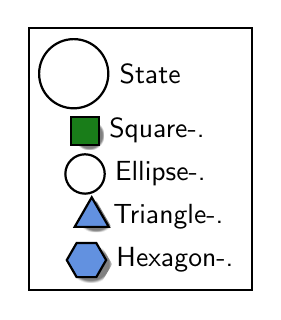
\begin{tikzpicture}
	[->,>=stealth',shorten >=2pt,node distance=3cm,
	thick,main node/.style={circle,draw,scale=0.25,transform canvas={scale=0.75},font=\sffamily\Small\bfseries},
	blacknode/.style={shape=circle, draw=black, line width=2},
	bluenode/.style={shape=circle, draw=blue, line width=2},
	greennode/.style={shape=circle, draw=green, line width=2},
	rednode/.style={shape=circle, draw=red, line width=2}
	]
	%-------Legend ------------------------------------------------------------	
	\matrix [draw,below left] at (current bounding box.south) {
		\node [state,label=right:State] {}; Description. \\
		\node [shapeSquare,label=right:Square-.] {}; \\
		\node [shapeEllipse,label=right:Ellipse-.] {}; \\
		\node [shapeTriangle,label=right:Triangle-.] {}; \\
		\node [shapeHexagon,label=right:Hexagon-.] {}; \\
	};
\end{tikzpicture}

\centering	
\begin{table}[H]\tiny
\caption{Gene/Protein/Enzymes Description and References}	
\begin{tabular}{r|p{3cm}|l}
\hline	
Gene/Protein & Description & Reference \\
\hline 
\hline 
\end{tabular}
\end{table}



\section{Mathematical Background}

\subsection{Equation Systems}

\begin{align*} 
\tiny
\frac{d^{\alpha_1}X_1(t)}{dt^{\alpha_1}} = a_{11} *X_1(t - \tau_1) + \\
a_{12} *\frac{X_1(t)^{\beta_1}}{(1-X_1(t - \tau_1))^{\beta_1}} - a_{15}X_1(t) + \\
\epsilon_1(t) \\
\frac{d^{\alpha_1}X_2(t)}{dt^{\alpha_1}} = a_{21} *X_2(t - \tau_2) + \\
a_{22} *\frac{X_2(t)^{\beta_1}}{(1-X_2(t - \tau_2))^{\beta_1}} - a_{25}X_2(t) + \\
\epsilon_2(t) \\ \\
\frac{d^{\alpha_1}X_3(t)}{dt^{\alpha_1}} = a_{31} *X_3(t - \tau_3) + \\
a_{32} *\frac{X_3(t)^{\beta_1}}{(1-X_3(t - \tau_3))^{\beta_1}} - a_{35}X_3(t) + \\
\epsilon_3(t) \\ \\
\frac{d^{\alpha_1}X_4(t)}{dt^{\alpha_1}} = a_{41} *X_4(t - \tau_4) + \\
a_{42} *\frac{X_4(t)^{\beta_1}}{(1-X_4(t - \tau_4))^{\beta_1}} - a_{45}X_4(t) + \\
\epsilon_4(t) \\ \\
\frac{d^{\alpha_1}X_5(t)}{dt^{\alpha_1}} = a_{51} *X_5(t - \tau_5) + \\
a_{52} *\frac{X_5(t)^{\beta_1}}{(1-X_5(t - \tau_5))^{\beta_1}} - a_{55}X_5(t) + \\
\epsilon_5(t) \\
\end{align*}

\subsubsection{Parameter Table}

\begin{table}[h]\footnotesize
	\caption{Parameter Description and Value}
	\begin{tabular}{rllp{2cm}l}
		\hline	
		Parameter & Value & Interval & Description & Reference \\
		\hline 
		a11 & 0 & [0,1] & Equation 1 & \cite{key1}
		a12 & 0 & [0,1] & Equation 1 & \cite{key1}
		a13 & 0 & [0,1] & Equation 1 & \cite{key1}
		a14 & 0 & [0,1] & Equation 1 & \cite{key1}
		a15 & 0 & [0,1] & Equation 1 & \cite{key1}
		\hline
		a21 & 0 & [0,1] & Equation 2 & \cite{key1}
		a22 & 0 & [0,1] & Equation 2 & \cite{key1}
		a23 & 0 & [0,1] & Equation 2 & \cite{key1}
		a24 & 0 & [0,1] & Equation 2 & \cite{key1}
		a25 & 0 & [0,1] & Equation 2 & \cite{key1}
		\hline
		a31 & 0 & [0,1] & Equation 3 & \cite{key1}
		a32 & 0 & [0,1] & Equation 3 & \cite{key1}
		a33 & 0 & [0,1] & Equation 3 & \cite{key1}
		a34 & 0 & [0,1] & Equation 3 & \cite{key1}
		a35 & 0 & [0,1] & Equation 3 & \cite{key1}
		\hline
		a41 & 0 & [0,1] & Equation 4 & \cite{key1}
		a42 & 0 & [0,1] & Equation 4 & \cite{key1}
		a43 & 0 & [0,1] & Equation 4 & \cite{key1}
		a44 & 0 & [0,1] & Equation 4 & \cite{key1}
		a45 & 0 & [0,1] & Equation 4 & \cite{key1}
		\hline
		a51 & 0 & [0,1] & Equation 5 & \cite{key1}
		a52 & 0 & [0,1] & Equation 5 & \cite{key1}
		a53 & 0 & [0,1] & Equation 5 & \cite{key1}
		a54 & 0 & [0,1] & Equation 5 & \cite{key1}
		a55 & 0 & [0,1] & Equation 5 & \cite{key1}
		\hline
		$\tau_1$ & 1 & [1,2] & Equation 1 & \cite{key1}
		$\tau_2$ & 1 & [1,2] & Equation 2 & \cite{key1}
		$\tau_3$ & 1 & [1,2] & Equation 3 & \cite{key1}
		$\tau_4$ & 1 & [1,2] & Equation 4 & \cite{key1}
		$\tau_5$ & 1 & [1,2] & Equation 5 & \cite{key1}
		\hline
		$\alpha_1$ & 1 & (0,2] & Equation 1 & \cite{key1}
		$\alpha_2$ & 1 & (0,2] & Equation 2 & \cite{key1}
		$\alpha_3$ & 1 & (0,2] & Equation 3 & \cite{key1}
		$\alpha_4$ & 1 & (0,2] & Equation 4 & \cite{key1}
		$\alpha_5$ & 1 & (0,2] & Equation 5 & \cite{key1}
		\hline
		$\beta_1$ & 1 & (0,2] & Equation 1 & \cite{key1}
		$\beta_2$ & 1 & (0,2] & Equation 2 & \cite{key1}
		$\beta_3$ & 1 & (0,2] & Equation 3 & \cite{key1}
		$\beta_4$ & 1 & (0,2] & Equation 4 & \cite{key1}
		$\beta_5$ & 1 & (0,2] & Equation 5 & \cite{key1}
	\end{tabular}	
\end{table}




\subsubsection{Group A}

\begin{align*} 
\tiny
\frac{d^{\alpha_1}X_1(t)}{dt^{\alpha_1}} = a_{11} *X_1(t - \tau_1) + \\
a_{12} *\frac{X_1(t)^{\beta_1}}{(1-X_1(t - \tau_1))^{\beta_1}} - a_{15}X_1(t) + \\
\epsilon_1(t) \\
\frac{d^{\alpha_1}X_2(t)}{dt^{\alpha_1}} = a_{21} *X_2(t - \tau_2) + \\
a_{22} *\frac{X_2(t)^{\beta_1}}{(1-X_2(t - \tau_2))^{\beta_1}} - a_{25}X_2(t) + \\
\epsilon_2(t) \\ \\
\frac{d^{\alpha_1}X_3(t)}{dt^{\alpha_1}} = a_{31} *X_3(t - \tau_3) + \\
a_{32} *\frac{X_3(t)^{\beta_1}}{(1-X_3(t - \tau_3))^{\beta_1}} - a_{35}X_3(t) + \\
\epsilon_3(t) \\ \\
\frac{d^{\alpha_1}X_4(t)}{dt^{\alpha_1}} = a_{41} *X_4(t - \tau_4) + \\
a_{42} *\frac{X_4(t)^{\beta_1}}{(1-X_4(t - \tau_4))^{\beta_1}} - a_{45}X_4(t) + \\
\epsilon_4(t) \\ \\
\frac{d^{\alpha_1}X_5(t)}{dt^{\alpha_1}} = a_{51} *X_5(t - \tau_5) + \\
a_{52} *\frac{X_5(t)^{\beta_1}}{(1-X_5(t - \tau_5))^{\beta_1}} - a_{55}X_5(t) + \\
\epsilon_5(t) \\
\end{align*}

\subsubsection{Parameter Table}

\begin{table}[h]\footnotesize
	\caption{Parameter Description and Value}
	\begin{tabular}{rllp{2cm}l}
		\hline	
		Parameter & Value & Interval & Description & Reference \\
		\hline 
		a11 & 0 & [0,1] & Equation 1 & \cite{key1}
		a12 & 0 & [0,1] & Equation 1 & \cite{key1}
		a13 & 0 & [0,1] & Equation 1 & \cite{key1}
		a14 & 0 & [0,1] & Equation 1 & \cite{key1}
		a15 & 0 & [0,1] & Equation 1 & \cite{key1}
		\hline
		a21 & 0 & [0,1] & Equation 2 & \cite{key1}
		a22 & 0 & [0,1] & Equation 2 & \cite{key1}
		a23 & 0 & [0,1] & Equation 2 & \cite{key1}
		a24 & 0 & [0,1] & Equation 2 & \cite{key1}
		a25 & 0 & [0,1] & Equation 2 & \cite{key1}
		\hline
		a31 & 0 & [0,1] & Equation 3 & \cite{key1}
		a32 & 0 & [0,1] & Equation 3 & \cite{key1}
		a33 & 0 & [0,1] & Equation 3 & \cite{key1}
		a34 & 0 & [0,1] & Equation 3 & \cite{key1}
		a35 & 0 & [0,1] & Equation 3 & \cite{key1}
		\hline
		a41 & 0 & [0,1] & Equation 4 & \cite{key1}
		a42 & 0 & [0,1] & Equation 4 & \cite{key1}
		a43 & 0 & [0,1] & Equation 4 & \cite{key1}
		a44 & 0 & [0,1] & Equation 4 & \cite{key1}
		a45 & 0 & [0,1] & Equation 4 & \cite{key1}
		\hline
		a51 & 0 & [0,1] & Equation 5 & \cite{key1}
		a52 & 0 & [0,1] & Equation 5 & \cite{key1}
		a53 & 0 & [0,1] & Equation 5 & \cite{key1}
		a54 & 0 & [0,1] & Equation 5 & \cite{key1}
		a55 & 0 & [0,1] & Equation 5 & \cite{key1}
		\hline
		$\tau_1$ & 1 & [1,2] & Equation 1 & \cite{key1}
		$\tau_2$ & 1 & [1,2] & Equation 2 & \cite{key1}
		$\tau_3$ & 1 & [1,2] & Equation 3 & \cite{key1}
		$\tau_4$ & 1 & [1,2] & Equation 4 & \cite{key1}
		$\tau_5$ & 1 & [1,2] & Equation 5 & \cite{key1}
		\hline
		$\alpha_1$ & 1 & (0,2] & Equation 1 & \cite{key1}
		$\alpha_2$ & 1 & (0,2] & Equation 2 & \cite{key1}
		$\alpha_3$ & 1 & (0,2] & Equation 3 & \cite{key1}
		$\alpha_4$ & 1 & (0,2] & Equation 4 & \cite{key1}
		$\alpha_5$ & 1 & (0,2] & Equation 5 & \cite{key1}
		\hline
		$\beta_1$ & 1 & (0,2] & Equation 1 & \cite{key1}
		$\beta_2$ & 1 & (0,2] & Equation 2 & \cite{key1}
		$\beta_3$ & 1 & (0,2] & Equation 3 & \cite{key1}
		$\beta_4$ & 1 & (0,2] & Equation 4 & \cite{key1}
		$\beta_5$ & 1 & (0,2] & Equation 5 & \cite{key1}
	\end{tabular}	
\end{table}



\subsubsection{Group B}

\begin{align*} 
\tiny
\frac{d^{\alpha_1}X_1(t)}{dt^{\alpha_1}} = a_{11} *X_1(t - \tau_1) + \\
a_{12} *\frac{X_1(t)^{\beta_1}}{(1-X_1(t - \tau_1))^{\beta_1}} - a_{15}X_1(t) + \\
\epsilon_1(t) \\
\frac{d^{\alpha_1}X_2(t)}{dt^{\alpha_1}} = a_{21} *X_2(t - \tau_2) + \\
a_{22} *\frac{X_2(t)^{\beta_1}}{(1-X_2(t - \tau_2))^{\beta_1}} - a_{25}X_2(t) + \\
\epsilon_2(t) \\ \\
\frac{d^{\alpha_1}X_3(t)}{dt^{\alpha_1}} = a_{31} *X_3(t - \tau_3) + \\
a_{32} *\frac{X_3(t)^{\beta_1}}{(1-X_3(t - \tau_3))^{\beta_1}} - a_{35}X_3(t) + \\
\epsilon_3(t) \\ \\
\frac{d^{\alpha_1}X_4(t)}{dt^{\alpha_1}} = a_{41} *X_4(t - \tau_4) + \\
a_{42} *\frac{X_4(t)^{\beta_1}}{(1-X_4(t - \tau_4))^{\beta_1}} - a_{45}X_4(t) + \\
\epsilon_4(t) \\ \\
\frac{d^{\alpha_1}X_5(t)}{dt^{\alpha_1}} = a_{51} *X_5(t - \tau_5) + \\
a_{52} *\frac{X_5(t)^{\beta_1}}{(1-X_5(t - \tau_5))^{\beta_1}} - a_{55}X_5(t) + \\
\epsilon_5(t) \\
\end{align*}

\subsubsection{Parameter Table}

\begin{table}[h]\footnotesize
	\caption{Parameter Description and Value}
	\begin{tabular}{rllp{2cm}l}
		\hline	
		Parameter & Value & Interval & Description & Reference \\
		\hline 
		a11 & 0 & [0,1] & Equation 1 & \cite{key1}
		a12 & 0 & [0,1] & Equation 1 & \cite{key1}
		a13 & 0 & [0,1] & Equation 1 & \cite{key1}
		a14 & 0 & [0,1] & Equation 1 & \cite{key1}
		a15 & 0 & [0,1] & Equation 1 & \cite{key1}
		\hline
		a21 & 0 & [0,1] & Equation 2 & \cite{key1}
		a22 & 0 & [0,1] & Equation 2 & \cite{key1}
		a23 & 0 & [0,1] & Equation 2 & \cite{key1}
		a24 & 0 & [0,1] & Equation 2 & \cite{key1}
		a25 & 0 & [0,1] & Equation 2 & \cite{key1}
		\hline
		a31 & 0 & [0,1] & Equation 3 & \cite{key1}
		a32 & 0 & [0,1] & Equation 3 & \cite{key1}
		a33 & 0 & [0,1] & Equation 3 & \cite{key1}
		a34 & 0 & [0,1] & Equation 3 & \cite{key1}
		a35 & 0 & [0,1] & Equation 3 & \cite{key1}
		\hline
		a41 & 0 & [0,1] & Equation 4 & \cite{key1}
		a42 & 0 & [0,1] & Equation 4 & \cite{key1}
		a43 & 0 & [0,1] & Equation 4 & \cite{key1}
		a44 & 0 & [0,1] & Equation 4 & \cite{key1}
		a45 & 0 & [0,1] & Equation 4 & \cite{key1}
		\hline
		a51 & 0 & [0,1] & Equation 5 & \cite{key1}
		a52 & 0 & [0,1] & Equation 5 & \cite{key1}
		a53 & 0 & [0,1] & Equation 5 & \cite{key1}
		a54 & 0 & [0,1] & Equation 5 & \cite{key1}
		a55 & 0 & [0,1] & Equation 5 & \cite{key1}
		\hline
		$\tau_1$ & 1 & [1,2] & Equation 1 & \cite{key1}
		$\tau_2$ & 1 & [1,2] & Equation 2 & \cite{key1}
		$\tau_3$ & 1 & [1,2] & Equation 3 & \cite{key1}
		$\tau_4$ & 1 & [1,2] & Equation 4 & \cite{key1}
		$\tau_5$ & 1 & [1,2] & Equation 5 & \cite{key1}
		\hline
		$\alpha_1$ & 1 & (0,2] & Equation 1 & \cite{key1}
		$\alpha_2$ & 1 & (0,2] & Equation 2 & \cite{key1}
		$\alpha_3$ & 1 & (0,2] & Equation 3 & \cite{key1}
		$\alpha_4$ & 1 & (0,2] & Equation 4 & \cite{key1}
		$\alpha_5$ & 1 & (0,2] & Equation 5 & \cite{key1}
		\hline
		$\beta_1$ & 1 & (0,2] & Equation 1 & \cite{key1}
		$\beta_2$ & 1 & (0,2] & Equation 2 & \cite{key1}
		$\beta_3$ & 1 & (0,2] & Equation 3 & \cite{key1}
		$\beta_4$ & 1 & (0,2] & Equation 4 & \cite{key1}
		$\beta_5$ & 1 & (0,2] & Equation 5 & \cite{key1}
	\end{tabular}	
\end{table}



\subsubsection{Group C}

\begin{align*} 
\tiny
\frac{d^{\alpha_1}X_1(t)}{dt^{\alpha_1}} = a_{11} *X_1(t - \tau_1) + \\
a_{12} *\frac{X_1(t)^{\beta_1}}{(1-X_1(t - \tau_1))^{\beta_1}} - a_{15}X_1(t) + \\
\epsilon_1(t) \\
\frac{d^{\alpha_1}X_2(t)}{dt^{\alpha_1}} = a_{21} *X_2(t - \tau_2) + \\
a_{22} *\frac{X_2(t)^{\beta_1}}{(1-X_2(t - \tau_2))^{\beta_1}} - a_{25}X_2(t) + \\
\epsilon_2(t) \\ \\
\frac{d^{\alpha_1}X_3(t)}{dt^{\alpha_1}} = a_{31} *X_3(t - \tau_3) + \\
a_{32} *\frac{X_3(t)^{\beta_1}}{(1-X_3(t - \tau_3))^{\beta_1}} - a_{35}X_3(t) + \\
\epsilon_3(t) \\ \\
\frac{d^{\alpha_1}X_4(t)}{dt^{\alpha_1}} = a_{41} *X_4(t - \tau_4) + \\
a_{42} *\frac{X_4(t)^{\beta_1}}{(1-X_4(t - \tau_4))^{\beta_1}} - a_{45}X_4(t) + \\
\epsilon_4(t) \\ \\
\frac{d^{\alpha_1}X_5(t)}{dt^{\alpha_1}} = a_{51} *X_5(t - \tau_5) + \\
a_{52} *\frac{X_5(t)^{\beta_1}}{(1-X_5(t - \tau_5))^{\beta_1}} - a_{55}X_5(t) + \\
\epsilon_5(t) \\
\end{align*}

\subsubsection{Parameter Table}

\begin{table}[h]\footnotesize
	\caption{Parameter Description and Value}
	\begin{tabular}{rllp{2cm}l}
		\hline	
		Parameter & Value & Interval & Description & Reference \\
		\hline 
		a11 & 0 & [0,1] & Equation 1 & \cite{key1}
		a12 & 0 & [0,1] & Equation 1 & \cite{key1}
		a13 & 0 & [0,1] & Equation 1 & \cite{key1}
		a14 & 0 & [0,1] & Equation 1 & \cite{key1}
		a15 & 0 & [0,1] & Equation 1 & \cite{key1}
		\hline
		a21 & 0 & [0,1] & Equation 2 & \cite{key1}
		a22 & 0 & [0,1] & Equation 2 & \cite{key1}
		a23 & 0 & [0,1] & Equation 2 & \cite{key1}
		a24 & 0 & [0,1] & Equation 2 & \cite{key1}
		a25 & 0 & [0,1] & Equation 2 & \cite{key1}
		\hline
		a31 & 0 & [0,1] & Equation 3 & \cite{key1}
		a32 & 0 & [0,1] & Equation 3 & \cite{key1}
		a33 & 0 & [0,1] & Equation 3 & \cite{key1}
		a34 & 0 & [0,1] & Equation 3 & \cite{key1}
		a35 & 0 & [0,1] & Equation 3 & \cite{key1}
		\hline
		a41 & 0 & [0,1] & Equation 4 & \cite{key1}
		a42 & 0 & [0,1] & Equation 4 & \cite{key1}
		a43 & 0 & [0,1] & Equation 4 & \cite{key1}
		a44 & 0 & [0,1] & Equation 4 & \cite{key1}
		a45 & 0 & [0,1] & Equation 4 & \cite{key1}
		\hline
		a51 & 0 & [0,1] & Equation 5 & \cite{key1}
		a52 & 0 & [0,1] & Equation 5 & \cite{key1}
		a53 & 0 & [0,1] & Equation 5 & \cite{key1}
		a54 & 0 & [0,1] & Equation 5 & \cite{key1}
		a55 & 0 & [0,1] & Equation 5 & \cite{key1}
		\hline
		$\tau_1$ & 1 & [1,2] & Equation 1 & \cite{key1}
		$\tau_2$ & 1 & [1,2] & Equation 2 & \cite{key1}
		$\tau_3$ & 1 & [1,2] & Equation 3 & \cite{key1}
		$\tau_4$ & 1 & [1,2] & Equation 4 & \cite{key1}
		$\tau_5$ & 1 & [1,2] & Equation 5 & \cite{key1}
		\hline
		$\alpha_1$ & 1 & (0,2] & Equation 1 & \cite{key1}
		$\alpha_2$ & 1 & (0,2] & Equation 2 & \cite{key1}
		$\alpha_3$ & 1 & (0,2] & Equation 3 & \cite{key1}
		$\alpha_4$ & 1 & (0,2] & Equation 4 & \cite{key1}
		$\alpha_5$ & 1 & (0,2] & Equation 5 & \cite{key1}
		\hline
		$\beta_1$ & 1 & (0,2] & Equation 1 & \cite{key1}
		$\beta_2$ & 1 & (0,2] & Equation 2 & \cite{key1}
		$\beta_3$ & 1 & (0,2] & Equation 3 & \cite{key1}
		$\beta_4$ & 1 & (0,2] & Equation 4 & \cite{key1}
		$\beta_5$ & 1 & (0,2] & Equation 5 & \cite{key1}
	\end{tabular}	
\end{table}


\subsection{Global Asymptotic Stability}
\subsection{Geometric Ergodicity}
\subsection{Existence of a Property Free Distribution}
\subsection{Convergence to Stationary Distribution with Density}
\subsection{Simulated Examples}

\section{Data: Gene/Protein/Enzyme}

\begin{table}[H]\centering
\begin{tabular}{p{1cm}p{1cm}p{1cm}p{1cm}p{1cm}p{1cm}p{4cm}}\
ID & A & B & C & D & E & F \\
\hline
\hline
\end{tabular}
\end{table}

\subsection{Cancer Pathway Genes}

\begin{table}[H]\centering
\begin{tabular}{p{1cm}p{1cm}p{1cm}p{1cm}p{1cm}p{1cm}p{4cm}}\
ID & A & B & C & D & E & F \\
\hline
\hline
\end{tabular}
\end{table}

\section{Signaling Transduction Network}

\begin{table}[H]\centering
\begin{tabular}{p{1cm}p{1cm}p{1cm}p{1cm}p{1cm}p{1cm}p{4cm}}\
ID & A & B & C & D & E & F \\
\hline
\hline
\end{tabular}
\end{table}

\subsection{Cellular Processes}

\subsection{Cell Cycle}

\begin{table}[H]\centering
\begin{tabular}{p{1cm}p{1cm}p{1cm}p{1cm}p{1cm}p{1cm}p{4cm}}\
ID & A & B & C & D & E & F \\
\hline
\hline
\end{tabular}
\end{table}

\subsection{Signal Transduction Network: Classification Node and Edge}

\begin{table}[H]\centering
\begin{tabular}{p{1cm}p{1cm}p{1cm}p{1cm}p{1cm}p{1cm}p{4cm}}\
ID & A & B & C & D & E & F \\
\hline
\hline
\end{tabular}
\end{table}

\subsection{Subset Networks A:B:C:D}

\begin{table}[H]\centering
\begin{tabular}{p{1cm}p{1cm}p{1cm}p{1cm}p{1cm}p{1cm}p{4cm}}\
ID & A & B & C & D & E & F \\
\hline
\hline
\end{tabular}
\end{table}

\subsubsection{Network Group A}

\begin{table}[H]\centering
\begin{tabular}{p{1cm}p{1cm}p{1cm}p{1cm}p{1cm}p{1cm}p{4cm}}\
Parameter & Name & Value & Interval & PDF & Sample & Reference \\
\hline
\hline
\end{tabular}
\end{table}

\subsubsection{Network Group B}

\begin{table}[H]\centering
\begin{tabular}{p{1cm}p{1cm}p{1cm}p{1cm}p{1cm}p{1cm}p{4cm}}\
Parameter & Name & Value & Interval & PDF & Sample & Reference \\
\hline
\hline
\end{tabular}
\end{table}

\subsubsection{Network Group C}

\begin{table}[H]\centering
\begin{tabular}{p{1cm}p{1cm}p{1cm}p{1cm}p{1cm}p{1cm}p{4cm}}\
Parameter & Name & Value & Interval & PDF & Sample & Reference \\
\hline
\hline
\end{tabular}
\end{table}

\subsubsection{Network Group D}

\begin{table}[H]\centering
\begin{tabular}{p{1cm}p{1cm}p{1cm}p{1cm}p{1cm}p{1cm}p{4cm}}\
Parameter & Name & Value & Interval & PDF & Sample & Reference \\
\hline
\hline
\end{tabular}
\end{table}

\section{Cell Lines}
\section{Design of Equations: Signal Network}
\subsection{Subset Networks A:B:C:D}

\begin{table}[H]\centering
\begin{tabular}{p{1cm}p{1cm}p{1cm}p{1cm}p{1cm}p{1cm}p{4cm}}\
Parameter & Name & Value & Interval & PDF & Sample & Reference \\
\hline
\hline
\end{tabular}
\end{table}

\section{Results}

\subsection{Mathematical Statistical Feature Sets}

\begin{table}[H]\centering
\begin{tabular}{p{1cm}p{1cm}p{1cm}p{1cm}p{1cm}p{1cm}p{4cm}}\
ID & A & B & C & D & E & F \\
\hline
\hline
\end{tabular}
\end{table}

\subsection{Equilibrium Analysis}

\begin{table}[H]\centering
\begin{tabular}{p{1cm}p{1cm}p{1cm}p{1cm}p{1cm}p{1cm}p{4cm}}\
ID & A & B & C & D & E & F \\
\hline
\hline
\end{tabular}
\end{table}

\subsection{Stability Theory and Analysis}

\subsection{Cell Cycle Timing, Orchestration, Coordination, and Duration}

\subsection{Network Group A}

\begin{table}[H]\centering
\begin{tabular}{p{1cm}p{1cm}p{1cm}p{1cm}p{1cm}p{1cm}p{4cm}}\
ID & A & B & C & D & E & F \\
\hline
\hline
\end{tabular}
\end{table}

\subsection{Figures}

\begin{figure}[H]
	\centering
	\begin{minipage}[b]{0.5\linewidth}
	%\includegraphics[scale=0.25]{Example_1_Figure_1.png}
	\end{minipage}\hfill
	\begin{minipage}[b]{0.5\linewidth}
	%\includegraphics[scale=0.25]{Example_1_Figure_2.png}
	\end{minipage}\hfill	
	\begin{minipage}[b]{0.5\linewidth}
	%\includegraphics[scale=0.25]{Example_1_Figure_3.png}
	\end{minipage}\hfill
	\begin{minipage}[b]{0.5\linewidth}
	%\includegraphics[scale=0.25]{Example_1_Figure_4.png}
	\end{minipage}\hfill
	\caption{1, 2, 3 and 4}
	\label{fig:Figure1}
\end{figure} 

\subsection{Network Group B}

\begin{table}[H]\centering
\begin{tabular}{p{1cm}p{1cm}p{1cm}p{1cm}p{1cm}p{1cm}p{4cm}}\
ID & A & B & C & D & E & F \\
\hline
\hline
\end{tabular}
\end{table}

\subsection{Figures}

\begin{figure}[H]
	\centering
	\begin{minipage}[b]{0.5\linewidth}
	%\includegraphics[scale=0.25]{Example_2_Figure_1.png}
	\end{minipage}\hfill
	\begin{minipage}[b]{0.5\linewidth}
	%\includegraphics[scale=0.25]{Example_2_Figure_2.png}
	\end{minipage}\hfill	
	\begin{minipage}[b]{0.5\linewidth}
	%\includegraphics[scale=0.25]{Example_2_Figure_3.png}
	\end{minipage}\hfill
	\begin{minipage}[b]{0.5\linewidth}
	%\includegraphics[scale=0.25]{Example_2_Figure_4.png}
	\end{minipage}\hfill
	\caption{1, 2, 3 and 4}
	\label{fig:Figure1}
\end{figure} 

\subsection{Network Group C}

\begin{table}[H]\centering
\begin{tabular}{p{1cm}p{1cm}p{1cm}p{1cm}p{1cm}p{1cm}p{4cm}}\
ID & A & B & C & D & E & F \\
\hline
\hline
\end{tabular}
\end{table}

\subsection{Figures}

\begin{figure}[H]
	\centering
	\begin{minipage}[b]{0.5\linewidth}
	%\includegraphics[scale=0.25]{Example_3_Figure_1.png}
	\end{minipage}\hfill
	\begin{minipage}[b]{0.5\linewidth}
	%\includegraphics[scale=0.25]{Example_3_Figure_2.png}
	\end{minipage}\hfill	
	\begin{minipage}[b]{0.5\linewidth}
	%\includegraphics[scale=0.25]{Example_3_Figure_3.png}
	\end{minipage}\hfill
	\begin{minipage}[b]{0.5\linewidth}
	%\includegraphics[scale=0.25]{Example_3_Figure_4.png}
	\end{minipage}\hfill
	\caption{1, 2, 3 and 4}
	\label{fig:Figure1}
\end{figure} 

\subsection{Network Group D}

\begin{table}[H]\centering
\begin{tabular}{p{1cm}p{1cm}p{1cm}p{1cm}p{1cm}p{1cm}p{4cm}}\
ID & A & B & C & D & E & F \\
\hline
\hline
\end{tabular}
\end{table}

\subsection{Figures}

\begin{figure}[H]
	\centering
	\begin{minipage}[b]{0.5\linewidth}
	%\includegraphics[scale=0.25]{Example_4_Figure_1.png}
	\end{minipage}\hfill
	\begin{minipage}[b]{0.5\linewidth}
	%\includegraphics[scale=0.25]{Example_4_Figure_2.png}
	\end{minipage}\hfill	
	\begin{minipage}[b]{0.5\linewidth}
	%\includegraphics[scale=0.25]{Example_4_Figure_3.png}
	\end{minipage}\hfill
	\begin{minipage}[b]{0.5\linewidth}
	%\includegraphics[scale=0.25]{Example_4_Figure_4.png}
	\end{minipage}\hfill
	\caption{1, 2, 3 and 4}
	\label{fig:Figure1}
\end{figure} 

\section{Classroom Discussion}

\bibliographystyle{plain}
\begin{thebibliography}{00}
\footnotesize	

\bibitem[1]{key1}Chiu, T.P., et al. 
GBshape: a genome browser database for DNA shape annotations. 
Nucleic Acids Res 2014.
	
\bibitem[2]{key2}Comoglio, F., et al. 
\newblock High-resolution profiling of Drosophila replication start sites reveals a DNA shape and chromatin signature of metazoan origins. 
\newblock Cell reports 2015;11(5):821-834.
	
\bibitem[3]{key3}Yang, L., et al. 
\newblock TFBSshape: a motif database for DNA shape features of transcription factor binding sites. 
\newblock Nucleic Acids Res 2014;42 (Database issue):D148-155.
	
\bibitem[4]{key1}Zhou, T., et al. 
\newblock DNAshape: a method for the high-throughput prediction ofDNA structural features on a genomic scale. 
\newblock Nucleic Acids Res 2013;41(Web Server issue):W56-62.

\bibitem[5]{key107}Myles Hollander and Douglas A. Wolfe (1973), 
\newblock Nonparametric Statistical Methods. 
\newblock New York: John Wiley and Sons. Pages 185–194 (Kendall and Spearman tests).

\bibitem[1]{key1} Leonid Berezansky, Jaromír Baštinec, Josef Diblík and Zdenek Šmarda
\newblock On a delay population model with quadratic nonlinearity 
\newblock Advances in Difference Equations 2012, 2012:230

\subsection{Differential Equations}

\bibitem[1]{key1}A New Approach and Solution Technique to Solve Time Fractional Nonlinear Reaction-Diffusion Equations
\bibitem[1]{key1}Stability Analysis of Fractional-Order Nonlinear Systems with Delay
\bibitem[1]{key1}Application of the Multistep Generalized Differential Transform Method to Solve a Time-Fractional Enzyme Kinetics
\bibitem[1]{key1}Wavelet Methods for Solving Fractional Order Differential Equations
\bibitem[1]{key1}Numerical Methods for Pricing American Options with Time-Fractional PDE Models
\bibitem[1]{key1}Application of Multistep Generalized Differential Transform Method for the Solutions of the Fractional-Order Chua System
\bibitem[1]{key1}Numerical Solution of Some Types of Fractional Optimal Control Problems
\bibitem[1]{key1}An Efficient Series Solution for Fractional Differential Equations
\bibitem[1]{key1}Approximate Analytical Solution for Nonlinear System of Fractional Differential Equations by BPs Operational Matrices
\bibitem[1]{key1}Numerical Solution for Complex Systems of Fractional Order
\bibitem[1]{key1}Stability Analysis of Fractional-Order Nonlinear Systems with Delay
\bibitem[1]{key1}Numerical Study for Time Delay Multistrain Tuberculosis Model of Fractional Order
\bibitem[1]{key1}A Numerical Method for Solving Fractional Differential Equations by Using Neural Network
\bibitem[1]{key1}Numerical Studies for Fractional-Order Logistic Differential Equation with Two Different Delays
\bibitem[1]{key1}Numerical Modeling of Fractional-Order Biological Systems
\bibitem[1]{key1}Numerical Solution of Some Types of Fractional Optimal Control Problems
\bibitem[1]{key1}A Numerical Method for Delayed Fractional-Order Differential Equations
\bibitem[1]{key1} New Insights into the Fractional Order Diffusion Equation Using Entropy and Kurtosis
\bibitem[1]{key1} DELAY DIFFERENTIAL EQUATIONS IN SINGLE SPECIES DYNAMICS
\bibitem[1]{key1} An Improved Artificial Bee Colony Algorithm Based on Elite Strategy and Dimension Learning
\bibitem[1]{key1}Operators of Fractional Calculus and Their Applications
\bibitem[1]{key1} Modelling Physiological and Pharmacological Control on Cell Proliferation to Optimise Cancer Treatments
\bibitem[1]{key1}Press, W. H., S. A. Teukolsky, W. T Vetterling, and B. P. Flannery (2007). 
\newblock Numerical Recipes: The Art of Numerical Computing. 
\newblock Third Edition, Cambridge University Press, New York.

\subsection{R Packages}

\bibitem[100]{key1000}R Core Team (2015). 
\newblock R: A language and environment for statistical computing. R Foundation for Statistical Computing, Vienna, Austria.
\newblock URL https://www.R-project.org/.

\bibitem[101]{key1001} Hadley Wickham, Jim Hester and Romain Francois (2017). readr: Read
\newblock Rectangular Text Data. R package version 1.1.1.
\newblock https://CRAN.R-project.org/package=readr

\bibitem[102]{key1002} David B. Dahl (2016). 
\newblock xtable: Export Tables to LaTeX or HTML. R package version 1.8-2.
\newblock https://CRAN.R-project.org/package=xtable

\bibitem[103]{key1003}  Feinerer and Kurt Hornik (2017).
\newblock tm: Text Mining Package. 
\newblock R package version 0.7-1. https://CRAN.R-project.org/package=tm

\bibitem[104]{key1004}  Feinerer, Kurt Hornik, and David Meyer (2008). 
\newblock Text Mining Infrastructure in R. 
\newblock Journal of Statistical Software 25(5): 1-54. URL:http://www.jstatsoft.org/v25/i05/.

\bibitem[105]{key1005} B and Hornik K (2011).
\newblock topicmodels: An R Package for Fitting Topic Models.
\newblock Journal of Statistical Software, *40*(13), pp. 1-30. doi:10.18637/jss.v040.i13 (URL:http://doi.org/10.18637/jss.v040.i13).

\bibitem[106]{key1006} Ian Fellows (2014). 
\newblock wordcloud: Word Clouds. R package version 2.5.
\newblock https://CRAN.R-project.org/package=wordcloud

\bibitem[107]{key1007} Gagolewski M. and others (2017). 
\newblock R package stringi: Character string processing facilities. 
\newblock http://www.gagolewski.com/software/stringi/.DOI:10.5281/zenodo.32557

\bibitem[108]{key1008} Hadley Wickham (2017).
\newblock stringr: Simple, Consistent Wrappers for Common String Operations. 
\newblock R package version 1.2.0. https://CRAN.R-project.org/package=stringr

\subsubsection{Scientific Visualization}

\bibitem[201]{key2001}Michael J. Grayling (2014). 
\newblock phaseR:Phase Plane Analysis of One and Two Dimensional Autonomous ODE Systems. 
\newblock R package version 1.3. https://CRAN.R-project.org/package=phaseR

\bibitem[202]{key2002} Wei and Viliam Simko (2016).
\newblock corrplot: Visualization of a Correlation Matrix. 
\newblock R package version 0.77. https://CRAN.R-project.org/package=corrplot

\bibitem[203]{key2003} Soetaert (2017). 
\newblock plot3D: Plotting Multi-Dimensional Data. 
\newblock R package version 1.1.1. https://CRAN.R-project.org/package=plot3D

\bibitem[204]{key2004} Ligges, U. and Mächler, M. (2003).
\newblock Scatterplot3d - an R Package for Visualizing Multivariate Data.
\newblock Journal of Statistical Software 8(11), 1-20.

\bibitem[205]{key2005}Daniel Adler, Duncan Murdoch and others (2017). 
\newblock rgl: 3D Visualization Using OpenGL. 
\newblock R package version 0.98.1. https://CRAN.R-project.org/package=rgl

\bibitem[206]{key2006} Almende B.V., Benoit Thieurmel and Titouan Robert (2017). visNetwork:
\newblock Network Visualization using 'vis.js' Library. R package version 2.0.1.
\newblock https://CRAN.R-project.org/package=visNetwork

\bibitem[207]{key2007} Nicholas Hamilton (2017). 
\newblock ggtern: An Extension to 'ggplot2', for the Creation of Ternary Diagrams. 
\newblock R package version 2.2.1. https://CRAN.R-project.org/package=ggtern

\subsubsection{Mathematics and Statistics}

\bibitem[301]{key3001} Karline Soetaert, Jeff Cash and Francesca Mazzia (2016). 
\newblock deTestSet: Testset for Differential Equations. R package version 1.1.3.
\newblock http://CRAN.R-project.org/package=deTestSet

\bibitem[302]{key3002}Karline Soetaert, Thomas Petzoldt, R. Woodrow Setzer (2010). 
\newblock Solving Differential Equations in R: Package deSolve. 
\newblock Journal of Statistical Software, 33(9), 1--25. URL http://www.jstatsoft.org/v33/i09/ DOI 10.18637/jss.v033.i09

\bibitem[303]{key3003}Soetaert, Karline and Meysman, Filip, (2012).
\newblock Reactive transport in aquatic ecosystems: Rapid model prototyping in the open source software R
\newblock Environmental Modelling and Software, 32, 49-60.

\bibitem[304]{key3004}Soetaert K. and P.M.J. Herman (2009).  
\newblock A Practical Guide to Ecological Modelling. 
\newblock Using R as a Simulation Platform.  Springer, 372 pp.

\bibitem[305]{key3005}Soetaert K. (2009).  
\newblock rootSolve: Nonlinear root finding, equilibrium and steady-state analysis of ordinary differential equations.  
\newblock R-package version 1.6.

\bibitem[306]{key3006}Martin Becker and Stefan Klößner (2016). 
\newblock PearsonDS: Pearson Distribution System. 
\newblock R package version 0.98. http://CRAN.R-project.org/package=PearsonDS

\bibitem[307]{key3007}Csardi G, Nepusz T (2006).
\newblock The igraph software package for complex network research,
\newblock  InterJournal, Complex Systems 1695. 2006. http://igraph.org

\bibitem[308]{key3008} J. O. Ramsay, Hadley Wickham, Spencer Graves and Giles Hooker (2017). 
\newblock fda:Functional Data Analysis. 
\newblock R package version 2.4.7. https://CRAN.R-project.org/package=fda

\bibitem[309]{key3009} Antonio and Fabio Di Narzo (2013).
\newblock tseriesChaos: Analysis of nonlinear time series. 
\newblock R package version 0.1-13.https://CRAN.R-project.org/package=tseriesChaos

\bibitem[310]{key3010} Angelo Canty and Brian Ripley (2017). 
\newblock boot: Bootstrap R (S-Plus) Functions. 
\newblock R package version 1.3-20.

\bibitem[311]{key3011}Yves Tillé and Alina Matei (2016). 
\newblock sampling: Survey Sampling. 
\newblock R package version 2.8. https://CRAN.R-project.org/package=sampling

\bibitem[312]{key3012} Davison, A. C. and Hinkley, D. V. (1997) 
\newblock Bootstrap Methods and Their Applications. 
\newblock Cambridge University Press, Cambridge. ISBN 0-521-57391-2.

\bibitem[313]{key3013}Hans Werner Borchers (2017). 
\newblock pracma: Practical Numerical Math Functions. 
\newblock R package version 2.0.7. https://CRAN.R-project.org/package=pracma

\bibitem[314]{key3014}Marie Laure Delignette-Muller, Christophe Dutang (2015). 
\newblock fitdistrplus:An R Package for Fitting Distributions. 
\newblock Journal of Statistical Software, 64(4), 1-34. URL http://www.jstatsoft.org/v64/i04/.

\bibitem[315]{key3015} Scott Chasalow (2012). 
\newblock combinat: combinatorics utilities. 
\newblock R package version 0.0-8. https://CRAN.R-project.org/package=combinat

\bibitem[316]{key3016} C. Dutang, V. Goulet and M. Pigeon (2008). 
\newblock actuar: An R Package for Actuarial Science. 
\newblock Journal of Statistical Software, vol. 25, no. 7, 1-37. URL http://www.jstatsoft.org/v25/i07

\bibitem[317]{key3017} Douglas Bates and Martin Maechler (2017). 
\newblock Matrix: Sparse and Dense Matrix Classes and Methods. 
\newblock R package version 1.2-11.https://CRAN.R-project.org/package=Matrix

\bibitem[318]{key3018} Killick R, Haynes K and Eckley IA (2016).
\newblock changepoint: An R package for changepoint analysis. R package version
\newblock 2.2.2, <URL: https://CRAN.R-project.org/package=changepoint>.

\subsection{Genomics}

\bibitem[400]{key400} Kanehisa, Furumichi, M., Tanabe, M., Sato, Y., and Morishima, K.; 
\newblock KEGG: new perspectives on genomes, pathways, diseases and drugs. 
\newblock Nucleic Acids Res. 45, D353-D361 (2017).

\bibitem[401]{key401} Kanehisa, M., Sato, Y., Kawashima, M., Furumichi, M., and Tanabe, M.; 
\newblock KEGG as a reference resource for gene and protein annotation. 
\newblock Nucleic Acids Res. 44, D457-D462 (2016).

\bibitem[402]{key402} Kanehisa, M. and Goto, S.; 
\newblock KEGG: Kyoto Encyclopedia of Genes and Genomes. 
\newblock Nucleic Acids Res. 28, 27-30 (2000). 

\bibitem[403]{key403} Rouillard AD, Gundersen GW, Fernandez NF, Wang Z, Monteiro CD, McDermott MG, Ma'ayan A. 
\newblock The harmonizome: a collection of processed datasets gathered to serve and mine knowledge about genes and proteins. 
\newblock Database (Oxford). 2016 Jul 3;2016. pii: baw100. 

\bibitem[500]{key500} J. Timmer and M. König (1995): 
\newblock On generating power law noise. 
\newblock Astron. Astrophys. 300, 707-710.

\subsection{Bioconductor:Genomics}

\bibitem[4001]{key4001}D. Charif and J.R. Lobry (2007)
\newblock Structural approaches to sequence evolution: Molecules, networks, populations edited U. Bastolla and M. Porto and H.E. Roman and M. Vendruscolo 
\newblock New York: Springer Verlag

\bibitem[4002]{key4002} Jitao David Zhang and Stefan Wiemann (2009)
\newblock \emph{KEGGgraph: a graph approach to KEGG PATHWAY in R and Bioconductor}.
\newblock Bioinformatics, 25(11):1470--1471

\bibitem[4003]{key4003} Jitao David Zhang (2017). 
\newblock KEGGgraph: Application ExamplesR
\newblock package version 1.38.1.

\bibitem[4004]{key4004} David Winter (2017). 
\newblock rentrez: Entrez in R. 
\newblock R package version 1.1.0. https://CRAN.R-project.org/package=rentrez

\bibitem[4005]{key4005} H. Pagès, P. Aboyoun, R. Gentleman and S. DebRoy (2017).
\newblock Biostrings: String objects representing biological sequences, and matching algorithms. 
\newblock R package version 2.44.2.

\bibitem[4006]{key4006} Vesna Memisevic (2016). 
\newblock sysBio: A package for modeling biological systems. 
\newblock R package version 1.0.0. https://github.com/Vessy/sysBio

\bibitem[4007]{key4007} Philipp H Boersch-Supan, Sadie J Ryan, and Leah R Johnson (2016). 
\newblock deBInfer: Bayesian inference for dynamical models of biological systems in R. 
\newblock arXiv:1605.00021. URL https://arxiv.org/abs/1605.00021
	
\end{thebibliography}
\end{document}
